\documentclass{article}
\usepackage{amsmath, graphicx}
\graphicspath{ {./images/} }

\title{Ch. 7.2 -7.3 HW}
\author{Principles of Microeconomics}
\date{\today}

\begin{document}

\maketitle

\subsection*{Quick Quiz}

\begin{enumerate}
\setcounter{enumi}{3}

\item (c) --
	\begin{align*}
	PS_{Diego} &= 0 \text{ (because he doesn't take the job)} \\
	PS_{Emi} &= 300 - 200 = 100 \\
	PS_{Finn} &= 300 - 100 = 200 \\
	PS_{Mkt} &= 0 + 100 + 200 = 300
	\end{align*}
	
\item (b) -- Gavin's PS rises by \$100 because $PS = P - Cost$ and $P$ increased by 100. Hector's cost is higher than \$300 but lower than \$400 because he didn't work when the price was \$300 but he does when the price is \$400. That means his PS is 400 minus a number between 300 and 400, so his PS is between 0 and 100. Therefore, producer surplus increases 100 plus something between 0 and 100. 

\item (c) --

	\begin{center}
	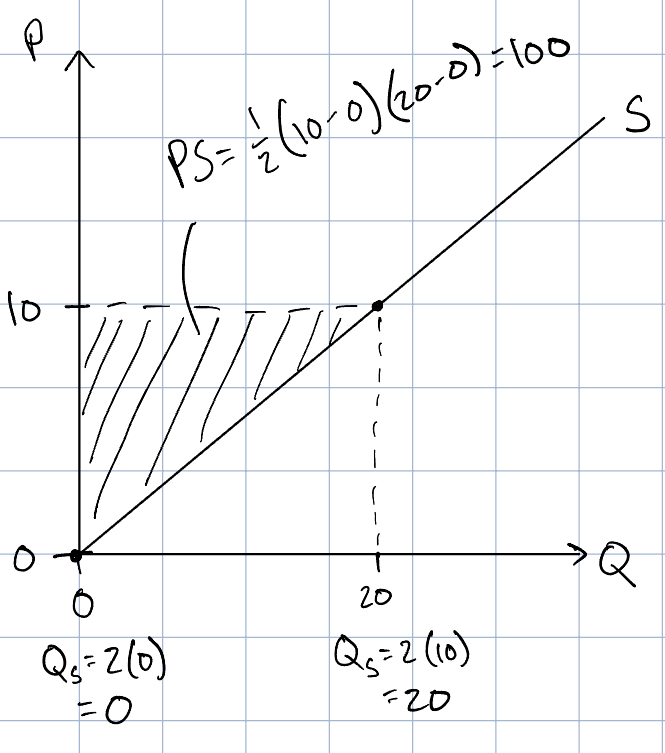
\includegraphics[width = 0.5\textwidth]{qq6}
	\end{center}

\end{enumerate}

\subsection*{Problems \& Applications}

\begin{enumerate}
\setcounter{enumi}{2}

\item When demand for French bread rises, the price rises. As a result, producer surplus increases.

	\begin{center}
	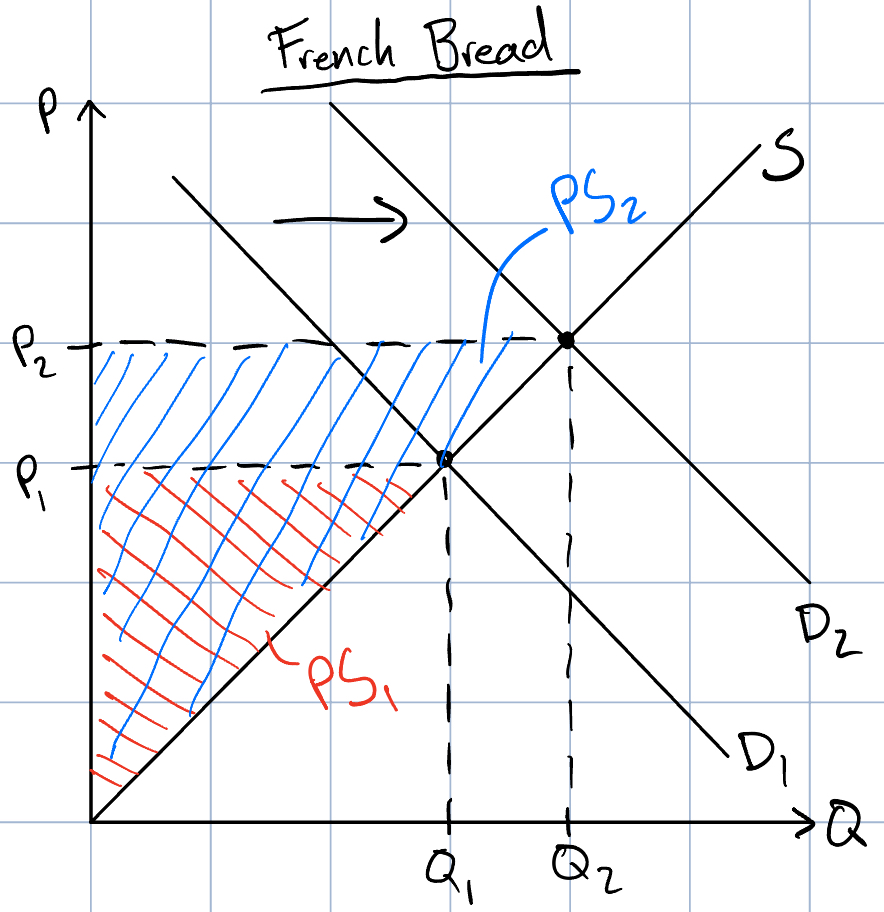
\includegraphics[width = 0.5\textwidth]{paa3_bread}
	\end{center}
	
	The quantity of french bread produced and sold increases, so there are more buyers of flour. That increases demand for flour which increases the price. As a result, producer surplus increases.
	
	\begin{center}
	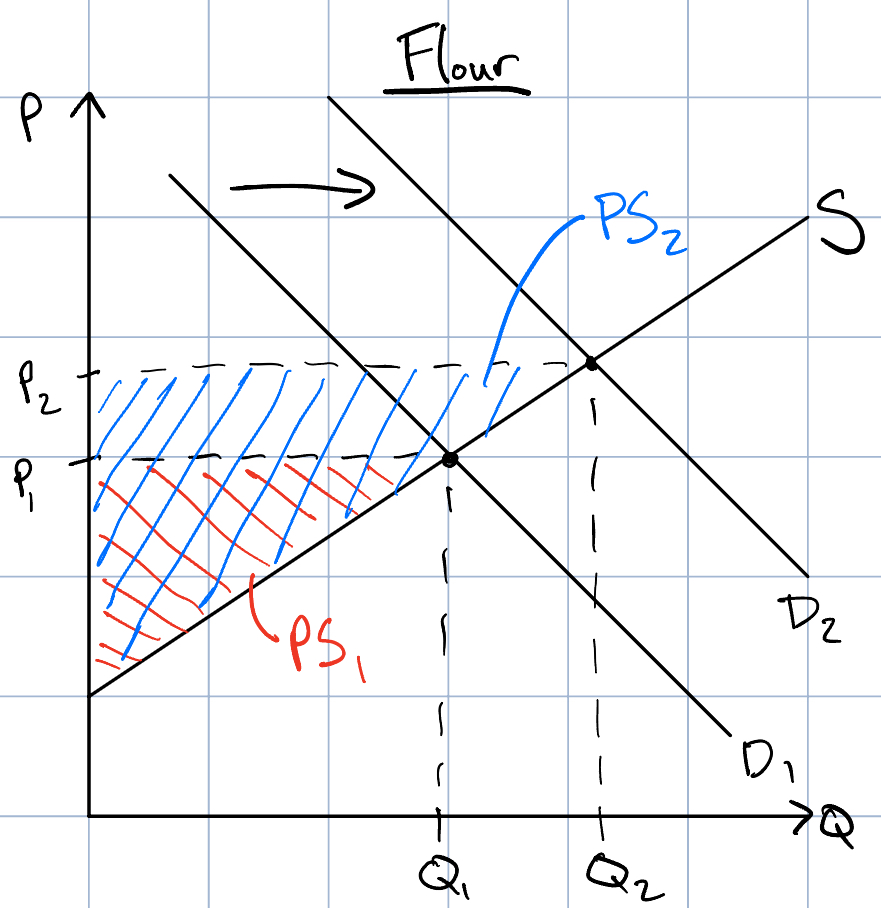
\includegraphics[width = 0.5\textwidth]{paa3_flour}
	\end{center}
	
\item

	\begin{enumerate}
	
	\item
		\begin{tabular}{c | c}
		$P$ & $Q_D$ \\
		\hline
		More than \$7 & 0 \\
		\$5 to \$7 & 1 \\
		\$3 to \$5 & 2 \\
		\$1 to \$3 & 3 \\
		Less than \$1 & 4
		\end{tabular}
		
	\item He buys 2 bottles of water. Consumer surplus is \$4.
	
	\item Quantity demanded increases to 3 bottles of water. Consumer surplus increases to \$9. 
	
		\begin{center}
		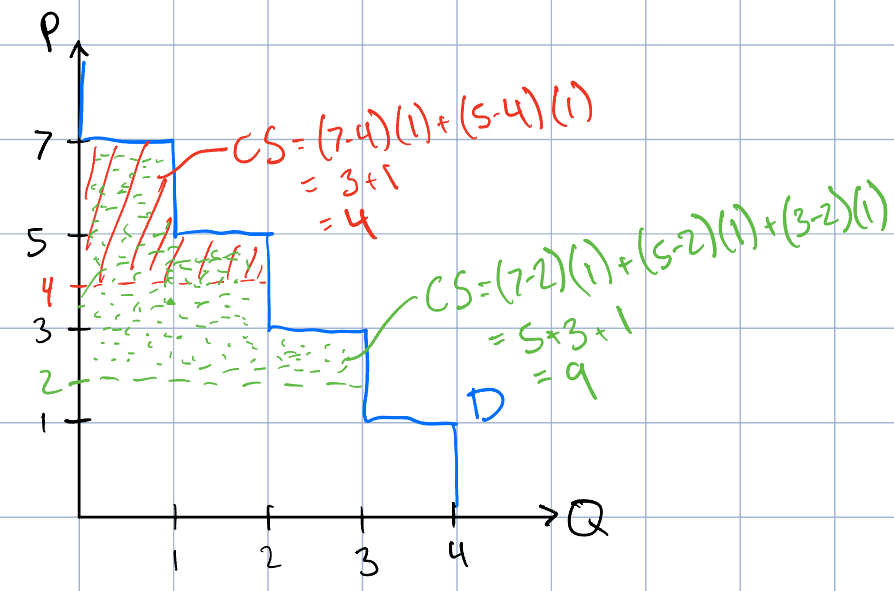
\includegraphics[width = 0.75\textwidth]{paa4}
		\end{center}
	
	\end{enumerate}
	
\item

	\begin{enumerate}
	
	\item
		\begin{tabular}{c | c}
		$P$ & $Q_S$ \\
		\hline
		Less than \$1 & 0 \\
		\$1 to \$3 & 1 \\
		\$3 to \$5 & 2 \\
		\$5 to \$7 & 3 \\
		More than \$7 & 4
		\end{tabular}
		
	\item He produces 2 bottles of water. His producer surplus is \$4.
	
	\item Quantity supplied increases to 3 bottles of water. His producer surplus increases to \$9.
	
		\begin{center}
		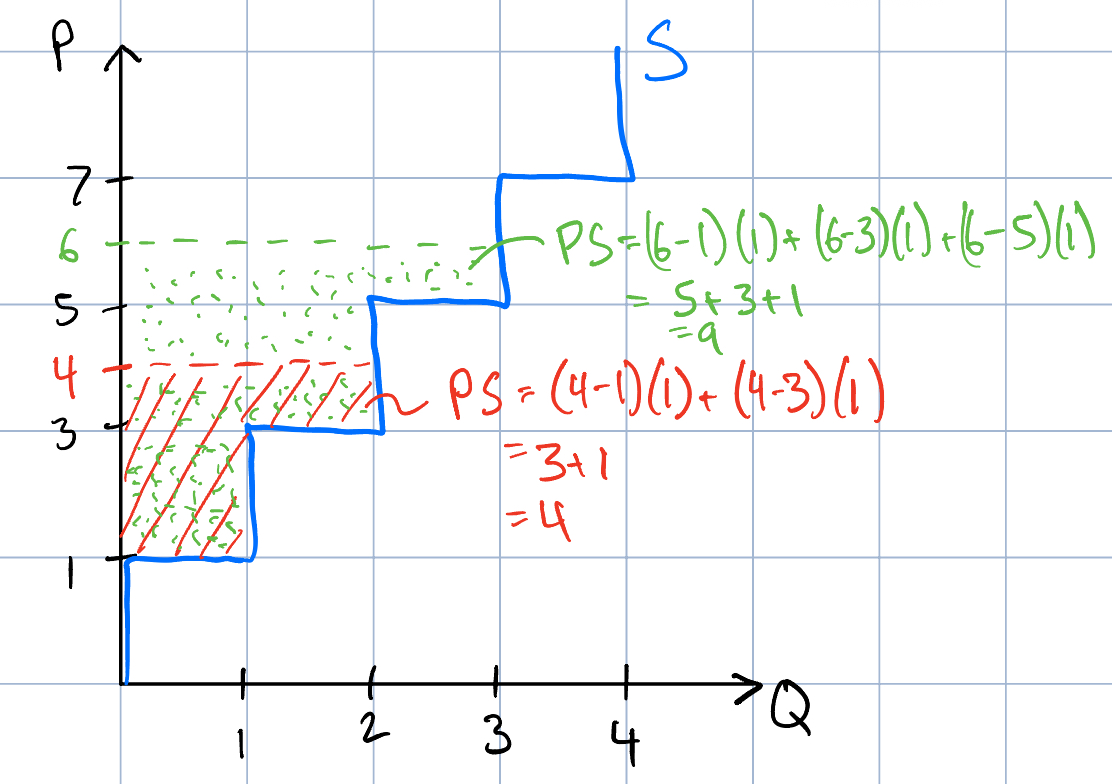
\includegraphics[width = 0.75\textwidth]{paa5}
		\end{center}
	
	\end{enumerate}
	
%\item
%
%	\begin{enumerate}
%	
%	\item 
%		\begin{tabular}{c | c | c}
%		$P$ & $Q_S$ & $Q_D$ \\
%		\hline
%		2 & 1 & 3 \\
%		4 & 2 & 2 \\
%		6 & 3 & 1 \\
%		\end{tabular}
%		
%		A price of \$4 brings supply and demand to equilibrium.
%		
%	\item From part (b) of \#4 and \#5, we know $CS = 4$ and $PS = 4$. Therefore, $TS = 4 + 4 = 8$.
%	
%	\item Total surplus would decrease to $3 + 3 = 6$.
%	
%		\begin{center}
%		\includegraphics[width = 0.5\textwidth]{paa6c}
%		\end{center} 
%		
%	\item Total surplus would decrease to $8 - 1 - 1 = 6$.
%	
%		\begin{center}
%		\includegraphics[width = 0.5\textwidth]{paa6d}
%		\end{center}
%	
%	\end{enumerate}

\end{enumerate}

\end{document}